\tocsection{\textbf{10/20/26 Lecture 16:} Gibbs Sampling in Practice and Empirical Bayes}

For MCMC, we choose $Q$ so $\pi(\theta) \propto_{\theta} \lambda(\theta)p_{\theta}(x)$, then $\tt{Dist}(\theta^{(t)}) \to \lambda(\theta \given x)$.\\

Recall the Gibbs sampler, where we build $\theta^{(t + 1)}$ by looping over each $\theta_j$, sampling from $\lambda(\theta_j \given \theta_{-j}, X)$.\\

Note that the Gibbs sampler is not necessarily irreducible. Consider the uniform distribution on the following set:
\begin{center}
    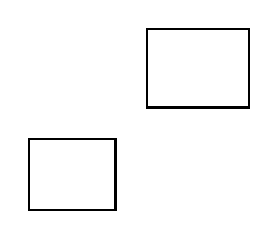
\begin{tikzpicture}
        \draw[thick] (0, 0) rectangle (1.1, 0.9);
        \draw[thick] (1.5, 1.3) rectangle (2.8, 2.3);
    \end{tikzpicture}
\end{center}
Then, changing only one coordinate at the time can never take us from one square to another, which implies that starting in one square will force us to stay there. \\

\textbf{Claim:} For the Gibbs sampler, if $\theta^{(t)} \sim \lambda(\theta \given X)$, then $\theta^{(t + 1)} \sim \lambda(\theta \given X)$.\\

\textbf{Proof:} Sampling $\theta_j$ from $\lambda(\theta_j \given \theta_{-j}, X)$ keeps us in the same distribution, so doing it $d$ times, we are fine. $\qed$

If $\theta, X$ follow a DAG model, we can write
\[ p(\theta, X) = \prod_{i = 1}^{d} p(\theta_i \given \tt{Pa}(\theta_i)) \prod_{i = 1}^{n} p(X_i \given \tt{Pa}(X_i)) \]
For instance, for the hierarchical model,
\begin{align*}
    p(\alpha, \beta, \theta_1, \ldots, \theta_m, X_1, \ldots, X_m) &= p(\alpha, \beta)\prod_{i = 1}^{m} p(\theta_i \given \alpha, \beta)\prod_{i = 1}^{m} p(x_i \given \theta_i)\\
    &\propto_{\theta_i} p(\theta_i \given \alpha, \beta)p(x_i \given \theta_i)
\end{align*}
\begin{center}
    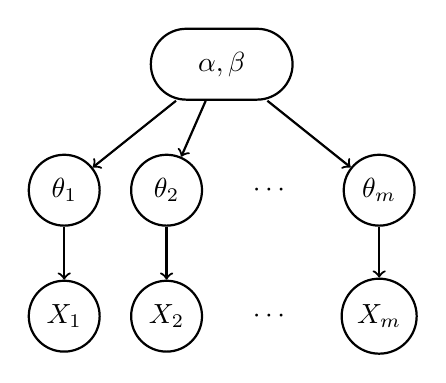
\begin{tikzpicture}[every node/.style = {circle, draw, thick, minimum size = 0.9cm}]
        \node[rectangle, rounded corners = 0.45cm, minimum width = 1.8cm] (ab) at (0, 0) {$\alpha, \beta$};
        \node (t1) at (-2, -1.6) {$\theta_1$};
        \node (t2) at (-0.7, -1.6) {$\theta_2$};
        \node[draw = none] at (0.6, -1.6) {$\cdots$};
        \node (tm) at (2, -1.6) {$\theta_m$};
        \node (x1) at (-2, -3.2) {$X_1$};
        \node (x2) at (-0.7, -3.2) {$X_2$};
        \node[draw = none] at (0.6, -3.2) {$\cdots$};
        \node (xm) at (2, -3.2) {$X_m$};
        \draw[->, thick] (ab) -- (t1);
        \draw[->, thick] (ab) -- (t2);
        \draw[->, thick] (ab) -- (tm);
        \draw[->, thick] (t1) -- (x1);
        \draw[->, thick] (t2) -- (x2);
        \draw[->, thick] (tm) -- (xm);
    \end{tikzpicture}
\end{center}

\subsection*{Gibbs Sampler in Practice}
\sectionspace

\textbf{Pro:} Given enough draws, we get the distribution.\\
\textbf{Con:} This may be a very long time.

\subsection*{Plots of Gibbs Samplers}
\sectionspace

\fig{0.4}{Lecture16Fig1}{}

\textbf{Idea:} We discard the entries in the \emph{burn-in period} and \emph{thin} the data by using only every couple samples.\\

\textbf{Using Samples:} Plot histograms for distribution, take mean for posterior mean. These give us an ``empirical estimate'' of the posterior.

\subsection*{Empirical Bayes}
\sectionspace

It's like Hierarchical Bayes, but we learn our hyperpriors:
\begin{align*}
    \alpha, \beta &\sim \lambda\\
    \theta_i \given \alpha, \beta &\iidsim \tt{Beta}(\alpha, \beta)\\
    X_i \given \theta_i, \alpha, \beta &\overset{\tt{ind}}{\sim} \Binom(n_i, \theta_i)
\end{align*}
Learn $\alpha$ and $\beta$ and hope $\lambda$ is irrelevant. Thus, we don't really need $\lambda$.\\

Recall our estimator was, under the hierarchical Bayes framework,
\[ \delta_i^{\tt{HB}}(X) = \E\left[\frac{X_i + \alpha}{n_i + \alpha + \beta} \given X\right] \]
where $\alpha, \beta$ are sampled from the posterior distribution $\lambda(\alpha, \beta \given x)$. For empirical Bayes, we will get
\[ \delta_i^{\tt{EB}}(X) = \frac{X_i + \hat{\alpha}}{n_i + \hat{\alpha} + \hat{\beta}} \]
where $\alpha, \beta$ are unknown and we estimate them.

\subsection*{Gaussian Sequence Model}
\sectionspace


Let $X \sim N_d(\theta, I_d) \iff X_i \overset{\tt{ind}}{\sim} N(\theta_i, 1)$.\\

\textbf{Goal:} Estimate $\theta \in \R^d$ via $\delta(X)$, and we want low $\tt{MSE}(\theta; \delta) = \E_{\theta}\norm{\theta - \delta(X)}^2$.\\

The reason this is good to study is the CLT.

\begin{example}{\textbf{Example:} CLT}
    If $X_1, \ldots, X_n \iidsim (\theta, \sigma^2 I_d)$, then
    \[ Z = \frac{1}{\sigma\sqrt{n}}\sum_{i} X_i \approx N\left(\frac{\sqrt{n}\theta}{\sigma}, I_d\right) \]
\end{example}

Now, the UMVU of the Gaussian sequence model is $X$. It's also the objective Bayes estimator and the MLE, which is nice.\\

\textbf{Linear Shrinkage Estimator:}
\[ \delta_{\zeta}(X) = (1 - \zeta)X \]
We saw this to be the Bayes estimator with $\theta_i \overset{\tt{ind}}{\sim} N(0, \tau^2)$, where $\zeta = \frac{1}{1 + \tau^2}$.\\

\textbf{Hierarchical Bayes:} If $\tau^2 \sim \lambda_0$, $\theta_i \given \tau^2 \iidsim N(0, \tau^2)$, we would get $\delta_{\zeta}$ with $\zeta = \E\left[\frac{1}{1 + \tau^2} \given X\right]$.\\

\textbf{Empirical Bayes:} Estimate $\tau^2$ or estimate $\zeta$ directly, so we get $\delta_{\hat{\zeta}}$ or $\delta_{\zeta}$ with $\zeta = \frac{1}{1 + \hat{\tau}^2}$. Since $X_i \given \tau^2 \iidsim N(0, 1 + \tau^2)$,
\[ \implies \norm{X}^2 \sim (1 + \tau^2)\chi_d^2 \implies \E[\norm{X}^2] = (1 + \tau^2)d \]

so estimate $\hat{\tau}^2 = \frac{\E[\norm{X}^2]}{d} - 1$, so $\hat{\zeta} = \frac{d}{\E[\norm{X}^2]}$.\\

\textbf{Note:} $\hat{\zeta}$ is positively biased by Jensen's, but it's still the MLE estimate.


